\chapter{Curriculum Learning for Infant-inspired Model Building: A Framework for Human-like Language Acquisition}
\label{chapter:CLIMB}

\newtcbox{\lightorangehighlight}{on line, colback=orange!10, boxrule=0.2mm, left=0.5mm, right=0.2mm, top=0.2mm, bottom=0.2mm}
\newtcbox{\darkorangehighlight}{on line, colback=orange!25, boxrule=0.2mm, left=0.5mm, right=0.2mm, top=0.2mm, bottom=0.2mm}

\newtcbox{\lightgreenhighlight}{on line, colback=green!10, boxrule=0.2mm, left=0.5mm, right=0.2mm, top=0.2mm, bottom=0.2mm}
\newtcbox{\darkgreenhighlight}{on line, colback=green!25, boxrule=0.2mm, left=0.5mm, right=0.2mm, top=0.2mm, bottom=0.2mm}
\newtcbox{\verydarkgreenhighlight}{on line, colback=green!40, boxrule=0.2mm, left=0.5mm, right=0.2mm, top=0.2mm, bottom=0.2mm}

\newtcbox{\lightpurplehighlight}{on line, colback=purple!10, boxrule=0.2mm, left=0.5mm, right=0.2mm, top=0.2mm, bottom=0.2mm}
\newtcbox{\darkpurplehighlight}{on line, colback=purple!25, boxrule=0.2mm, left=0.5mm, right=0.2mm, top=0.2mm, bottom=0.2mm}
\newtcbox{\verydarkpurplehighlight}{on line, colback=purple!40, boxrule=0.2mm, left=0.5mm, right=0.2mm, top=0.2mm, bottom=0.2mm}


While the background chapter established how human learning principles can inform language modeling, this chapter puts these ideas into practice through a concrete framework for curriculum learning. We present \climb (Curriculum Learning for Infant-inspired Model Building), a systematic approach to implementing developmentally plausible training protocols for language models. Our work is motivated by three key observations:

First, the current paradigm of language model training that relies on large datasets and computational resources stands in stark contrast to human language acquisition. Children acquire sophisticated language capabilities from only a few million words per year \citep{gilkerson2017mapping}, while state-of-the-art language models require trillions of tokens and extensive computational resources \citep{zhang2021need, zhao2023llmsurvey}. This discrepancy raises fundamental questions about the efficiency of current training approaches.

Second, conventional language model training differs from human learning in its structure: models operate on a predetermined static vocabulary and optimize a fixed objective on randomly shuffled data. In contrast, human language acquisition follows a carefully orchestrated progression: from babbling to simple utterances, and eventually to complex syntax and abstract meaning. This developmental trajectory suggests that structured learning protocols might enable more efficient model training.

Third, while curriculum learning has shown promise in various machine learning domains \citep{bengio2009curriculum}, its application to language modeling remains fragmented. Previous work has explored individual aspects such as vocabulary progression, data sequencing, or objective simplification but lacks a unified framework for implementing and evaluating these strategies, particularly in resource-constrained settings.

To address these challenges, we develop \climb within the context of the BabyLM Challenge \citep{warstadt2023babylm1}, which provides an ideal testbed for exploring cognitively plausible training protocols under strict data constraints (10 million words). Our framework systematically implements three curriculum dimensions:

\begin{itemize}
    \item \textbf{Vocabulary Curriculum:} Gradually expanding the model's lexicon, mirroring how children build their vocabulary from concrete nouns and verbs to more abstract terms.
    \item \textbf{Data Curriculum:} Structuring training data to progress from simpler to more complex linguistic structures, following the developmental trajectory observed in child language acquisition.
    \item \textbf{Objective Curriculum:} Evolving learning objectives from broad linguistic categories to specific token prediction, similar to how children first grasp word classes before mastering precise lexical distinctions.
\end{itemize}

Our work makes several key contributions:

\begin{enumerate}
    \item We establish a novel framework for categorizing and implementing curriculum learning strategies that simulate human language acquisition, providing a foundation for future research in cognitively inspired language modeling.
    
    \item Through extensive experimentation, we evaluate the effectiveness of different curriculum approaches under real-world constraints, offering concrete recommendations for when and how to apply specific curriculum strategies.
    
    \item We demonstrate that careful model and hyperparameter selection can yield strong performance even with limited data, with our vanilla models outperforming shared task baselines on grammatical knowledge (BLiMP) and approaching state-of-the-art performance on natural language understanding (SuperGLUE).
    
    \item We provide insights into the interaction between different curriculum dimensions, suggesting directions for developing more integrated approaches to curriculum learning in language modeling.
\end{enumerate}

The remainder of this chapter is organized as follows: Section 2 reviews the theoretical foundations of curriculum learning and its application to language modeling. Section 3 details our methodology, including the \climb framework and experimental setup. Section 4 presents our results and analysis, comparing different curriculum strategies and their combinations. Section 5 discusses the implications of our findings and directions for future work. Finally, Section 6 concludes with key insights and recommendations for implementing curriculum learning in language modeling.

\section{Methodology}

The work in this chapter is conducted within the context of the BabyLM Challenge \citep{warstadt2023babylm1}, which provides a constrained setting (10 million words) for exploring cognitively plausible training protocols. Before implementing our curriculum learning strategies, we first establish a strong baseline model and data processing pipeline. 

\subsection{Model Architecture and Training Setup}
All of our models are based on an 8-layer Transformer language model (\cref{subsec:baseline}) comparable to the BabyBERTa model \citep{huebner2021babyberta}. This architecture choice was motivated by the success of smaller models in low-resource settings, as demonstrated in the original BabyBERTa work. For all experiments, we leverage several key tools and frameworks to ensure robust and reproducible training. The Hugging Face Transformers library \citep{transformers} provides our model implementation, while Weights \& Biases \citep{wandb} enables comprehensive performance tracking and experiment monitoring. We use Hydra \citep{hydra} for experiment configuration management, allowing us to systematically explore different curriculum learning strategies. All training is conducted on a high performance computing cluster to ensure efficient model development and experimentation.

\subsection{Training Data}
\label{subsec:data}

\subsubsection{Data Source and Size}
We work exclusively with the training data provided in the \textsc{strict-small} track of the BabyLM challenge. This dataset is carefully constrained to 10 million words, compiled from 10 diverse corpora to ensure a representative sample of language use. Through our preprocessing pipeline, we reduce the initial 1,058,740 newline-delineated samples to 335,858 instances, corresponding to approximately 9.4 million words.\footnote{The word count is estimated by whitespace splitting, following the same metric used by the task organizers. When applying a tokenizer, the pre-processed dataset contains 11.7 million words (including punctuation) or 13.6 million subwords, reflecting the additional tokens introduced by subword tokenization.} This reduction in instances is primarily due to our concatenation strategy for shorter sequences, which we discuss in detail below.

\subsubsection{Data Preprocessing}
The diversity of our data sources (spanning books, subtitles, transcripts, and articles) necessitated careful curation to ensure consistency across corpora. Our preprocessing pipeline implements several key transformations. First, we standardize the text through lowercasing and punctuation normalization. We then apply regular expressions to standardize typographical conventions, ensuring consistent representation of numbers, dates, and special characters. The pipeline also removes extraneous content that could interfere with language modeling, including page numbers, bibliography entries, plain text tables, and one-word on-screen actions commonly found in subtitle data.

For transcribed speech corpora (with the exception of the British National Corpus), we implement a special concatenation strategy. Contiguous sections of five lines are combined into single data instances, addressing the challenge of relatively short sequence lengths in speech data. This approach helps maximize the effective use of our model's context window. Finally, at the point of model input, we join data segments to make full use of the available sequence length, which is set to 128 subtokens. This joining strategy is particularly important for maintaining the coherence of longer texts while staying within the model's context window constraints.

\subsubsection{Part-of-Speech Tagging}

While our preprocessing pipeline ensures consistent text formatting, we also need to capture linguistic structure to support our curriculum learning experiments. In particular, our vocabulary and objective curricula (Sections \cref{subsec:vocab-cl} and \cref{subsec:objective-cl}) rely on syntactic information to guide the learning process. However, the \textsc{strict-small} track's prohibition on external resources presented a unique challenge for implementing POS tagging, as we could not use supervised taggers.

\begin{wrapfigure}{r}{0.45\textwidth}
    \centering
    \small
    \begin{tabular}{lrrr}
    \toprule
    POS Tag & Precision & Recall & F1 \\
    \midrule
    NOUN & 0.786 & 0.790 & 0.788 \\
    DET & 0.820 & 0.772 & 0.795 \\
    CONJ & 0.969 & 0.821 & 0.895 \\
    NUM & 0.592 & 0.799 & 0.681 \\
    PRON & 0.592 & 0.962 & 0.733 \\   
    VERB & 0.816 & 0.823 & 0.819 \\
    PRT & 0.501 & 0.701 & 0.584 \\
    ADJ & 0.673 & 0.554 & 0.608 \\
    ADP & 0.842 & 0.888 & 0.864 \\
    PUNC & 0.944 & 0.960 & 0.952 \\
    \bottomrule
    \end{tabular}
    \caption{\label{tbl:unsupervised-pos-performance} Performance metrics of our unsupervised POS tagger compared to NLTK's supervised system.}
    \label{fig:unsupervised-pos-performance}
\end{wrapfigure}

To address this, we developed an unsupervised approach using the \texttt{anchor-features} algorithm \cite{stratos2016unsupervisedpos}, which identifies "anchor words" strongly associated with specific grammatical categories and uses these to learn a hidden Markov model (HMM). We ran this algorithm on the training dataset, and generated 30 clusters of features that each capture some latent syntactic information. We then manually mapped each cluster to a universal POS tag \cite{petrov2012universalpos}, with several clusters often mapping to the same grammatical category. Notably, our clustering approach failed to identify distinct groups for adverbs (ADV) and unknown tokens (X). \cref{fig:unsupervised-pos-performance} shows the full performance of our unsupervised POS tagger compared to NLTK's supervised system across all POS tags.

When evaluated against NLTK's supervised system \cite{bird2009natural}, our tagger showed strong performance on punctuation (F1: 0.952) and conjunctions (F1: 0.895), likely due to their consistent usage patterns. However, it struggled more with particles (F1: 0.584) and adjectives (F1: 0.608), which may have more variable usage patterns or semantic dependencies. These variations highlight the challenges of unsupervised grammatical category learning in low-resource settings.

\subsubsection{Data Availability and Observations}
To promote reproducibility and further research in this area, we provide our cleaned and tagged versions of the 10M word dataset on Hugging Face, along with the complete preprocessing scripts.\footnote{\url{https://huggingface.co/cambridge-climb}} This includes all the transformations described above, as well as the POS tagging pipeline. Interestingly, our experiments revealed that models trained on the raw, unprocessed data often outperformed those trained on our carefully preprocessed version. This counterintuitive finding, which we discuss in detail in \cref{sec:discussion}, suggests that the linguistic "noise" in raw data may actually provide valuable learning signals for language models, particularly in low-resource settings.

\subsection{Vanilla Models}
\label{subsec:baseline}

\begin{table*}
\centering
\small
\setlength{\tabcolsep}{4pt}  % Reduce column spacing
\begin{tabular}{l | rrrrr | rrrr}
\toprule
Model  & L & H & Hidden & Int. & Vocab & Steps & BLiMP & BLiMP. Supp & Perplexity \\
\midrule
Small  & 8 & 8 & 256 & 2,048   & 8,192   & 250K      & 75.43      & 61.14       & 9.46    \\
Medium & 10 & 10 & 500 & 2,000 & 8,192  & 156K      & 76.45      & 63.28        & 9.05  \\
Large  & 12 & 12 & 768 & 3,072 & 8,192   & 94K      & 75.80      & 60.83      & 9.34 \\[2mm]
\hline \\
Small  & 8 & 8 & 256 & 2,048   & 16,384  & 250K      & 76.16      & 60.85       & 13.80    \\
Medium & 10 & 10 & 500 & 2,000  & 16,384 & 94K      & 76.09      & 60.03        & 13.80     \\
Large  & 12 & 12 & 768 & 3,072 & 16,384  & 62K      & 75.08      & 63.45      & 14.22     \\
\bottomrule
\end{tabular}
\caption{\label{tbl:baseline-size-comparison} Our vanilla BabyBERTa-style models evaluated on original BLiMP and the BLiMP-like tasks prepared for BabyLM (BLiMP.Supp). Models are grouped by their vocabulary sizes. L denotes the number of Transformer layers and H the number of attention heads per layer. The Hidden dimension (Hidden) represents the size of token representations at each layer, while the Intermediate dimension (Int.) indicates the expanded dimension size in the feed-forward network (typically 4x the hidden dimension).}
\end{table*}

We investigate three different sizes of a vanilla Pre-Layer Norm RoBERTa model \cite{liu2019roberta} based on the BabyBERTa model \cite{huebner2021babyberta}: `small', `medium', and `large' -- \cref{tbl:baseline-size-comparison} lists the model configurations and presents the results for the different model sizes evaluated by perplexity, on BLiMP \cite{warstadt2020blimp} and on the supplementary BLiMP-like tasks issued by the BabyLM organizers (`Blimp.Supp'). We found the medium model with a small vocabulary size performed the best overall; however, the small model achieved similar results, and so to save on compute and keep to the restrained intentions of the \textsc{strict-small} track, we used the small model in our curriculum learning experiments.

\begin{wrapfigure}{r}{0.45\textwidth}
    \centering
    \small
    \begin{tabular}{lc}
    \toprule
         Parameter& Value\\
    \midrule
         Layer Norm EPS& 1e-5 \\
         Tie Word Embeddings & False \\
         Learning Rate & 0.001 \\
         Optimizer & AdamW \\
         Scheduler Type & Linear\\
         Max Steps & 400,000 \\
         Warm-up Steps & 100,000\\
         Per Device Batch Size & 32 \\
    \bottomrule
    \end{tabular}
    \caption{Hyperparameter settings which are constant across our vanilla models described in \cref{subsec:baseline}.}
    \label{tbl:baseline_hyperparams}
\end{wrapfigure}

We use Byte Pair Encoding (BPE) tokenization \cite{gage1994bpe} with a vocabulary of 8,192 because it yields better overall performance compared to a larger vocabulary of 16,384. The tokenizers we use in our experiments were trained on the cleaned data that we processed using the steps outlined in \ref{subsec:data}. In pilot experiments, we did not observe the benefits reported by \citet{huebner2021babyberta} from removing the unmasking procedure that is a standard component of the MLM objective \cite{devlin2019bert}, and therefore did not investigate this option further. In \cref{tbl:baseline_hyperparams} we report all of the hypereparemeters we use throughout our experiemnts.

All of the curriculum learning methods in the following sections were applied on top of our small vanilla BabyBERTa-style baseline. To isolate the effect of the curriculum-learning training process, we fixed the architecture of the model and the model hyper-parameters. We use an AdamW optimizer with linear scheduling \cite{loshchilov2019decoupled}.

\section{A Three-Dimensional Framework for Curriculum Learning}
Curriculum learning \cite{bengio2009curriculum} is a machine-learning paradigm which optimizes a model's performance by gradually increasing the difficulty of training over time according to a set schedule (a `curriculum') -- based on the idea that learning should proceed from easy to hard, inspired by the way that humans learn \cite{elman1993learning}.
Within the context of curriculum learning, one of the central questions is how to define and manipulate the difficulty of the learning process over the course of training. In a recent survey, \citet{soviany2022curriculum} decompose this challenge into two main sub-problems: determining a sorting mechanism to assess the difficulty of instances and developing a pacing function for increasing difficulty over time. 

\begin{table*}[H]
    \centering
    \small
    \begin{tabular}{lll}
    \toprule
    \textbf{Curriculum Type} & \textbf{Parameter} &\textbf{Variants} \\
    \midrule
     \multirow{2}{*}{Vocabulary} & Selection & frequency, word class, mixed \\
     & Pacing & linear, logarithmic \\
     \midrule
     \multirow{3}{*}{Data} & Difficulty & source, unigram perplexity, self-perplexity \\
     & Pacing & linear, logarithmic \\
     & Initial Perplexity & unigram, random \\
      \midrule
     \multirow{2}{*}{Objective} & Tasks & noun-verb prediction, POS prediction, MLM\\
     & Learning Setup & sequential, multitask \\
    \bottomrule
    \end{tabular}
    \caption{\label{tbl:configurations} Curriculum learning experiments overview}
\end{table*}

\subsection{Defining Curricula across Three Dimensions}
Previous work in curriculum learning typically focuses on difficulty from a data-centric perspective, however, we note that difficulty can arise from (at least) three major elements of training a neural model: the input representation, the data sampling, and the training process. We explore curriculum learning strategies across three distinct dimensions: the vocabulary, the order of training data, and the objective function.

\subsection{Vocabulary Curriculum}
\label{subsec:vocab-cl}

We propose a novel \textbf{vocabulary curriculum} that gradually expands the model's lexicon during training, inspired by how children build their vocabulary. While large language models typically begin training with a full, fixed vocabulary, children acquire language through a more progressive process, starting with a small vocabulary that expands rapidly at a rate of eight to ten words per day \cite{weizman2001lexical}. Moreover, children prioritize learning certain word classes before others, typically mastering verbs and nouns before progressing to more abstract parts of speech \cite{bergelson2015early}.

To simulate this developmental trajectory, we implement a curriculum that begins with a limited vocabulary (10\% of tokens) and gradually expands it over the course of training. During the initial stages, tokens not included in the active vocabulary are mapped to an unknown token (\textsc{UNK}) representation. The curriculum regime spans from 25,000 to 350,000 training steps, after which all vocabulary tokens become available for the final 50,000 steps of training.

We explore three strategies for selecting which tokens to include at each stage of the curriculum:

\begin{enumerate}
    \item \lightgreenhighlight{\textbf{Frequency-based selection} (Freq)} Tokens are chosen based on their frequency in the corpus, approximated using the BPE tokenizer's ID assignments (lower IDs correspond to more frequent tokens).
    
    \item \darkgreenhighlight{\textbf{Word class-based selection} (POS)} Tokens are selected according to their grammatical category, following a progression from lexical to functional classes as observed in child language acquisition \cite{bergelson2015early}: NOUN, VERB, ADJ, PRON, DET, ADP, NUM, CONJ, PRT, PNCT. All words within a given part-of-speech category are introduced simultaneously.
    
    \item \verydarkgreenhighlight{\textbf{Hybrid selection} (Hybrid)} We combine frequency and word class constraints by sorting words by their frequency within each part-of-speech category. This approach allows for more granular control over vocabulary expansion while maintaining the developmental progression of word classes.
\end{enumerate}

The rate at which the vocabulary expands is controlled by a pacing function. We experiment with both linear and logarithmic pacing functions, with the latter potentially better reflecting the rapid early vocabulary growth observed in children. \cref{fig:pacing_fn} illustrates how the percentage of unmasked vocabulary increases over the course of training under these different pacing regimes.

\begin{wrapfigure}{r}{0.45\textwidth}    
    \centering
    \small
    \renewcommand{\arraystretch}{1}
    \begin{tabular}{cl}
    \toprule
    \textbf{Difficulty} & \textbf{Corpora} \\
    \midrule
    1 & AO-CHILDES \\
    \midrule
    \multirow{2}{*}{2} & BNC Spoken \\
                           & Switchboard \\
    \midrule
    \multirow{2}{*}{3} & Open Subtitles \\
                           & QED \\
    \midrule
    \multirow{2}{*}{4} & CBT \\
                           & Children's Stories \\
    \midrule
    5 & Simple Wikipedia \\
    \midrule
    \multirow{2}{*}{6} & Wikipedia \\
                           & Gutenberg \\
    \bottomrule
    \end{tabular}
    \caption{\label{tbl:source_order} Difficulty levels assigned to each dataset, ordered from 1 (easiest, e.g., child-directed speech) to 6 (hardest, e.g., complex written texts).}
    \vspace{-2em} % Try -0.5em, -1em, or -2em as needed
\end{wrapfigure}

This approach represents, to our knowledge, the first systematic attempt at implementing a vocabulary curriculum in language model training, offering a more cognitively plausible alternative to the standard practice of training with a fixed, full vocabulary from the outset.

\subsection{Data Curriculum}
\label{subsec:data-cl}

We implement a \textbf{data curriculum} that structures the presentation of training instances to mirror how children learn language. Unlike conventional language model training, which typically presents randomly ordered data after minimal cleaning, our approach carefully sequences training instances based on their difficulty. This is motivated by the observation that the order of training instances can significantly impact model performance \citep{schluter2018data} and by the "Goldilocks effect" in human learning, where optimal learning occurs when stimuli are neither too easy nor too hard \cite{kidd2012goldilocks}. We explore two complementary approaches to determining instance difficulty:


\begin{enumerate}

    \item \lightpurplehighlight{\textbf{Source-based difficulty} (Source)} Following \citet{huebner2021babyberta}, we order datasets based on their source, considering spoken samples as 'easier' and written texts as 'harder'. This ordering reflects the natural progression of language acquisition, where children typically learn from spoken language before mastering written forms. We implement a six-level difficulty hierarchy (\cref{tbl:source_order}), ranging from child-directed speech (CHILDES) to complex written texts (Wikipedia, Gutenberg).

    \item \darkpurplehighlight{\textbf{Static perplexity-based difficulty} (Static PPX)} While source-based difficulty provides a useful heuristic, it fails to capture the variation in complexity within each corpus. To address this limitation, we implement a more fine-grained approach using perplexity as a model-intrinsic metric of instance difficulty. Perplexity measures how well a language model predicts a sequence of words, with lower perplexity indicating that the model finds the sequence more predictable and thus potentially easier to learn from. 

    We use perplexity as a model-intrinsic metric of instance difficulty. Perplexity measures how well a language model predicts a sequence of words, with lower perplexity indicating that the model finds the sequence more predictable and thus potentially easier to learn from. We explore two distinct approaches to perplexity-based difficulty assessment. The first approach uses a static assessment, where we employ a unigram language model to evaluate perplexity once at the start of training. This method provides a simple, computationally efficient baseline that captures basic frequency patterns in the data. The unigram model's perplexity scores remain fixed throughout training, offering a consistent difficulty ranking of instances that reflects the inherent complexity of the text based on word frequencies.

    \item \verydarkpurplehighlight{\textbf{Dynamic perplexity-based difficulty} (Dynamic PPX)} The second approach implements a dynamic assessment strategy, where we periodically re-evaluate perplexity using the current model state. We perform these reassessments every 25,000 training steps, allowing the difficulty assessment to evolve with the model's growing capabilities. This dynamic approach better reflects the "Goldilocks effect" in learning, where optimal progress occurs when instances are neither too easy nor too hard \citep{kidd2012goldilocks}. As the model learns and develops, instances that were initially challenging may become more manageable, while others may reveal hidden complexities that weren't apparent at first.

    The dynamic approach presents several unique challenges that require careful consideration. The primary challenge arises at the start of training, when the model lacks sufficient exposure to provide meaningful perplexity scores. We address this initialization challenge through two complementary strategies. First, we can use a separately trained unigram model for initial perplexity evaluation, which provides a reasonable starting point for difficulty assessment (Dynamic PPX-U). Alternatively, we can begin with random sampling for the first 25,000 steps before switching to model-based perplexity evaluation (Dynamic PPX-R).

    The periodic reassessment of perplexity every 25,000 steps creates an adaptive curriculum that evolves with the model's capabilities. This approach allows us to identify instances that have become too easy (exhibiting low perplexity) and potentially deprioritize them in the training schedule. Simultaneously, we can maintain focus on instances that remain challenging (showing high perplexity) and discover instances that have moved into the "Goldilocks zone" of optimal difficulty for the current model state.

\end{enumerate}

\subsection{Objective Curriculum}
\label{subsec:objective-cl}

We develop an \textbf{objective curriculum} that evolves the learning task from broad linguistic categories to specific token prediction, mirroring how children progress from understanding word classes to mastering precise lexical distinctions. This approach is motivated by the observation that human language learning is guided by interactions with other agents (e.g., adult caregivers, siblings) who help shape the learning process. In machine learning, these interactions are modeled through the objective function that guides the model's optimization.

The standard approach to language model training uses masked language modeling (MLM), which has proven highly successful for training Transformer networks \citep{devlin2019bert}. However, psycholinguistic research suggests that MLM may not be cognitively plausible as an approximation of child language acquisition \citep{caucheteux2023evidence}. The MLM objective presents a challenging discriminative classification task, requiring the model to predict a masked token's identity from the entire vocabulary (an $N$-way classification problem). This stands in contrast to how children learn, where they first develop sensitivity to distributional patterns and gradually learn to recognize lexical categories before mastering specific word forms \citep{alishahi2010computational, gleitman1990structural}.

To better align with this developmental trajectory, we implement a curriculum that gradually increases the specificity of the learning objective. We begin with broader linguistic categories and progressively narrow down to specific token prediction. This approach is inspired by recent work that simplifies classification tasks by reducing the number of possible classes from $N$ to $K$ (where $K << N$). Previous research has explored mapping rare words to hypernyms \citep{bai2022better} or replacing words with part-of-speech tags \citep{wang2023language} or syntactic dependency relations \citep{cui2022lert}. These approaches significantly reduce task difficulty by working with a smaller set of categories.

In our implementation, we use the unsupervised POS tagger to estimate word classes and experiment with two levels of classification granularity:
\begin{enumerate}
    \item A three-way classification distinguishing between VERB, NOUN, and OTHER categories
    \item A more detailed ten-way classification using universal POS tags
\end{enumerate}

We explore two strategies for implementing this curriculum:

\begin{enumerate}
    \item \lightorangehighlight{\textbf{Sequential learning} (Seq)} We first train the model to predict word classes, then transition to the full MLM objective. This approach mirrors the developmental progression observed in children, where they first learn to distinguish between major word classes before mastering specific lexical items.
    
    \item \darkorangehighlight{\textbf{Multi-task learning} (MT)} We train the model to simultaneously predict both word classes and specific tokens, with separate task heads and optimizers for each objective. This approach allows the model to benefit from both coarse-grained and fine-grained learning signals throughout training.
\end{enumerate}

The psycholinguistic literature remains divided on how exactly word learning progresses from memorizing specific lexical items to developing generalized representations of word classes \citep{clark2015first}. Our framework provides a flexible approach to studying this progression by enabling systematic investigation of how different objective functions affect the acquisition of linguistic knowledge. By varying the timing and combination of learning objectives, we can explore different hypotheses about the relationship between category learning and specific word acquisition in language development.

This objective curriculum represents a novel approach to making language model training more cognitively plausible while maintaining the benefits of the MLM objective. By starting with broader linguistic categories and gradually increasing specificity, we aim to create a learning trajectory that better reflects human language acquisition while potentially improving the model's ability to generalize from limited training data.

\subsection{Pacing Functions} 

\begin{wrapfigure}{l}{0.50\textwidth}
    \centering
    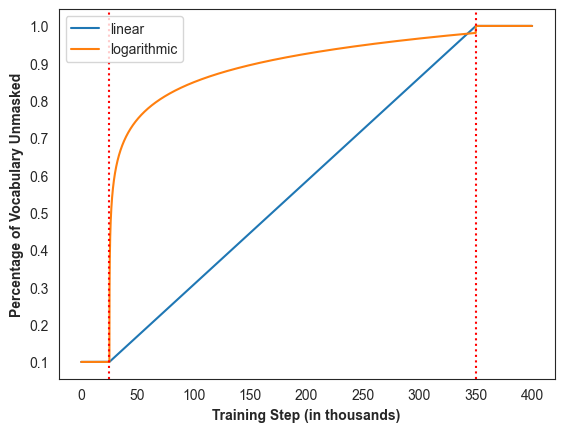
\includegraphics[width=0.45\textwidth]{chapters/climb/figures/pacing_fns.png}
    \caption{Illustration of the linear and logarithmic pacing functions used in our vocabulary curriculum experiments. The red dotted lines denote the curriculum regime, during which the percentage of unmasked words available to the model grows.}
    \label{fig:pacing_fn}
\end{wrapfigure}

Once a notion of difficulty is set, a pacing function is needed to govern how quickly the model will progress from training on easier examples to training on harder ones \citep{wu2021when}.

We experiment with two different pacing functions: linear and logarithmic. Linear pacing functions involve a steady and consistent advancement through the curriculum. This approach ensures a gradual increase in difficulty over time. Logarithmic pacing functions, on the other hand, emphasize early exposure to ``easier'' concepts, with diminishing increments as the model's capabilities are assumed to increase. Both pacing functions have been proposed in the broader curriculum learning literature \citep{bai2022better, li2021curriculum, wu2021when}. In \cref{fig:pacing_fn} we illustrate the two pacing functions for the vocabulary curriculum.

\begin{figure}[htbp]
    \centering
    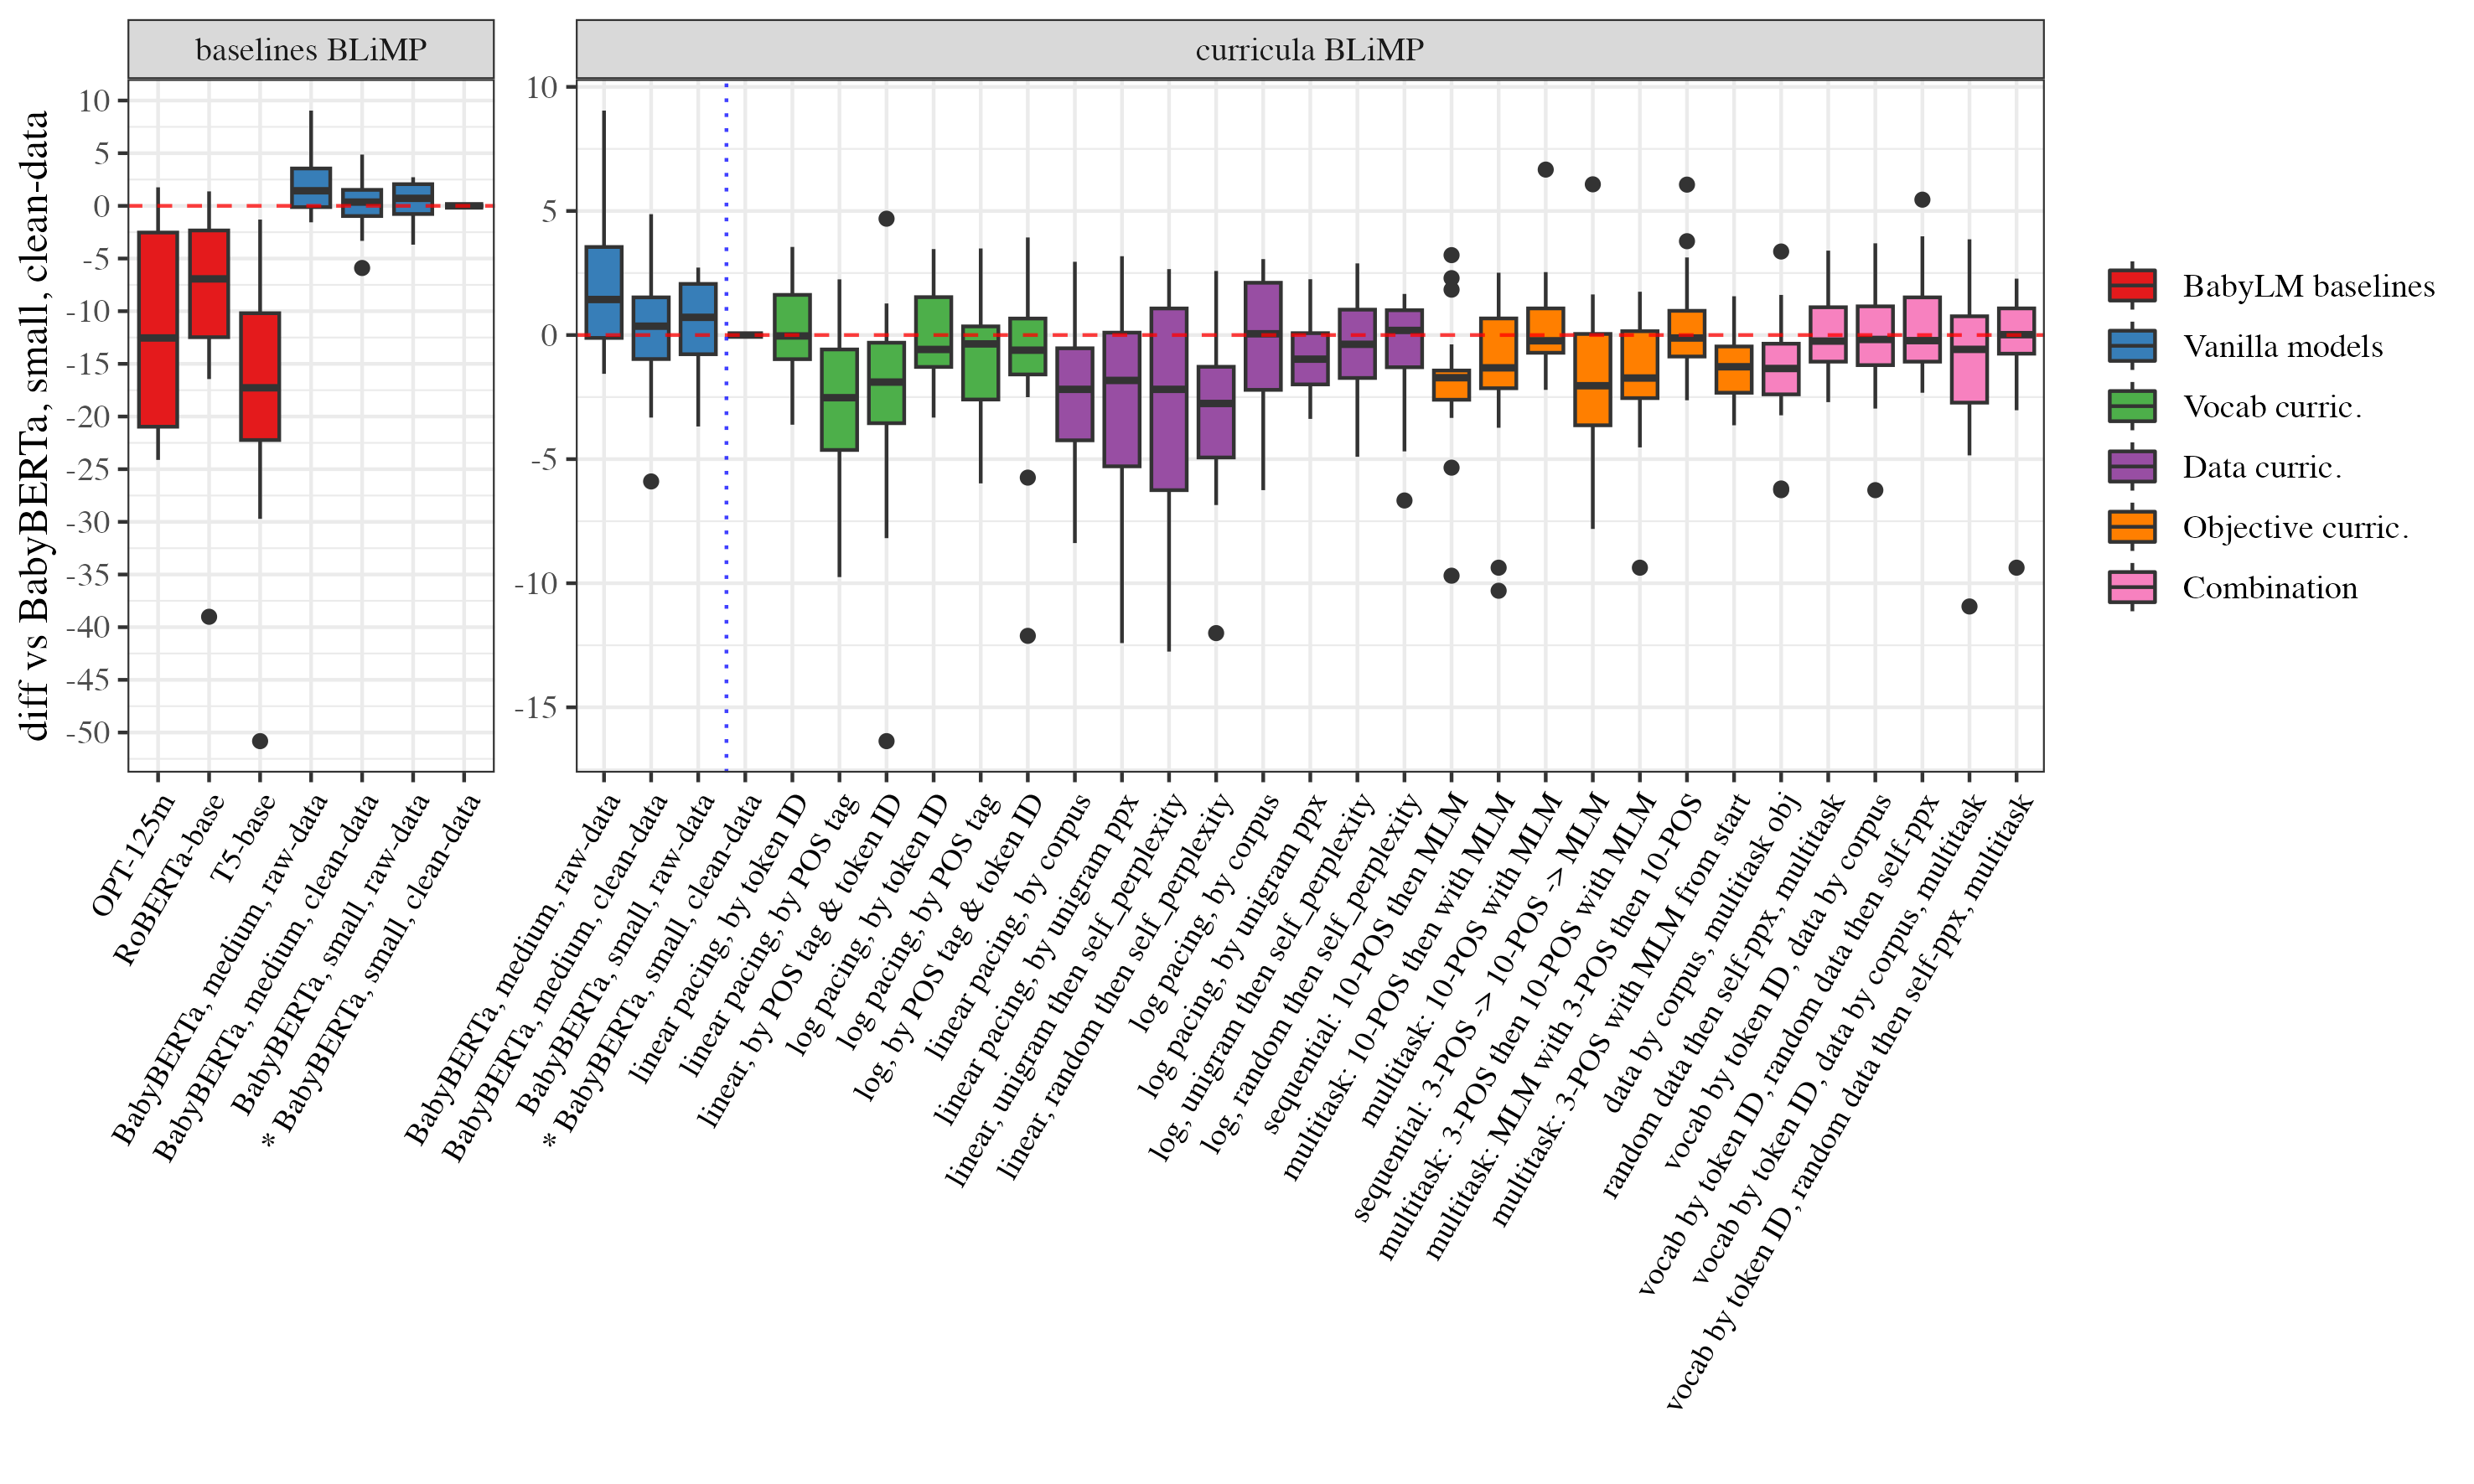
\includegraphics[width=0.9\textwidth]{chapters/climb/figures/babylm_blimp_diffs_boxplots.png}
    \vspace{1em}  % Add some vertical space between figures
    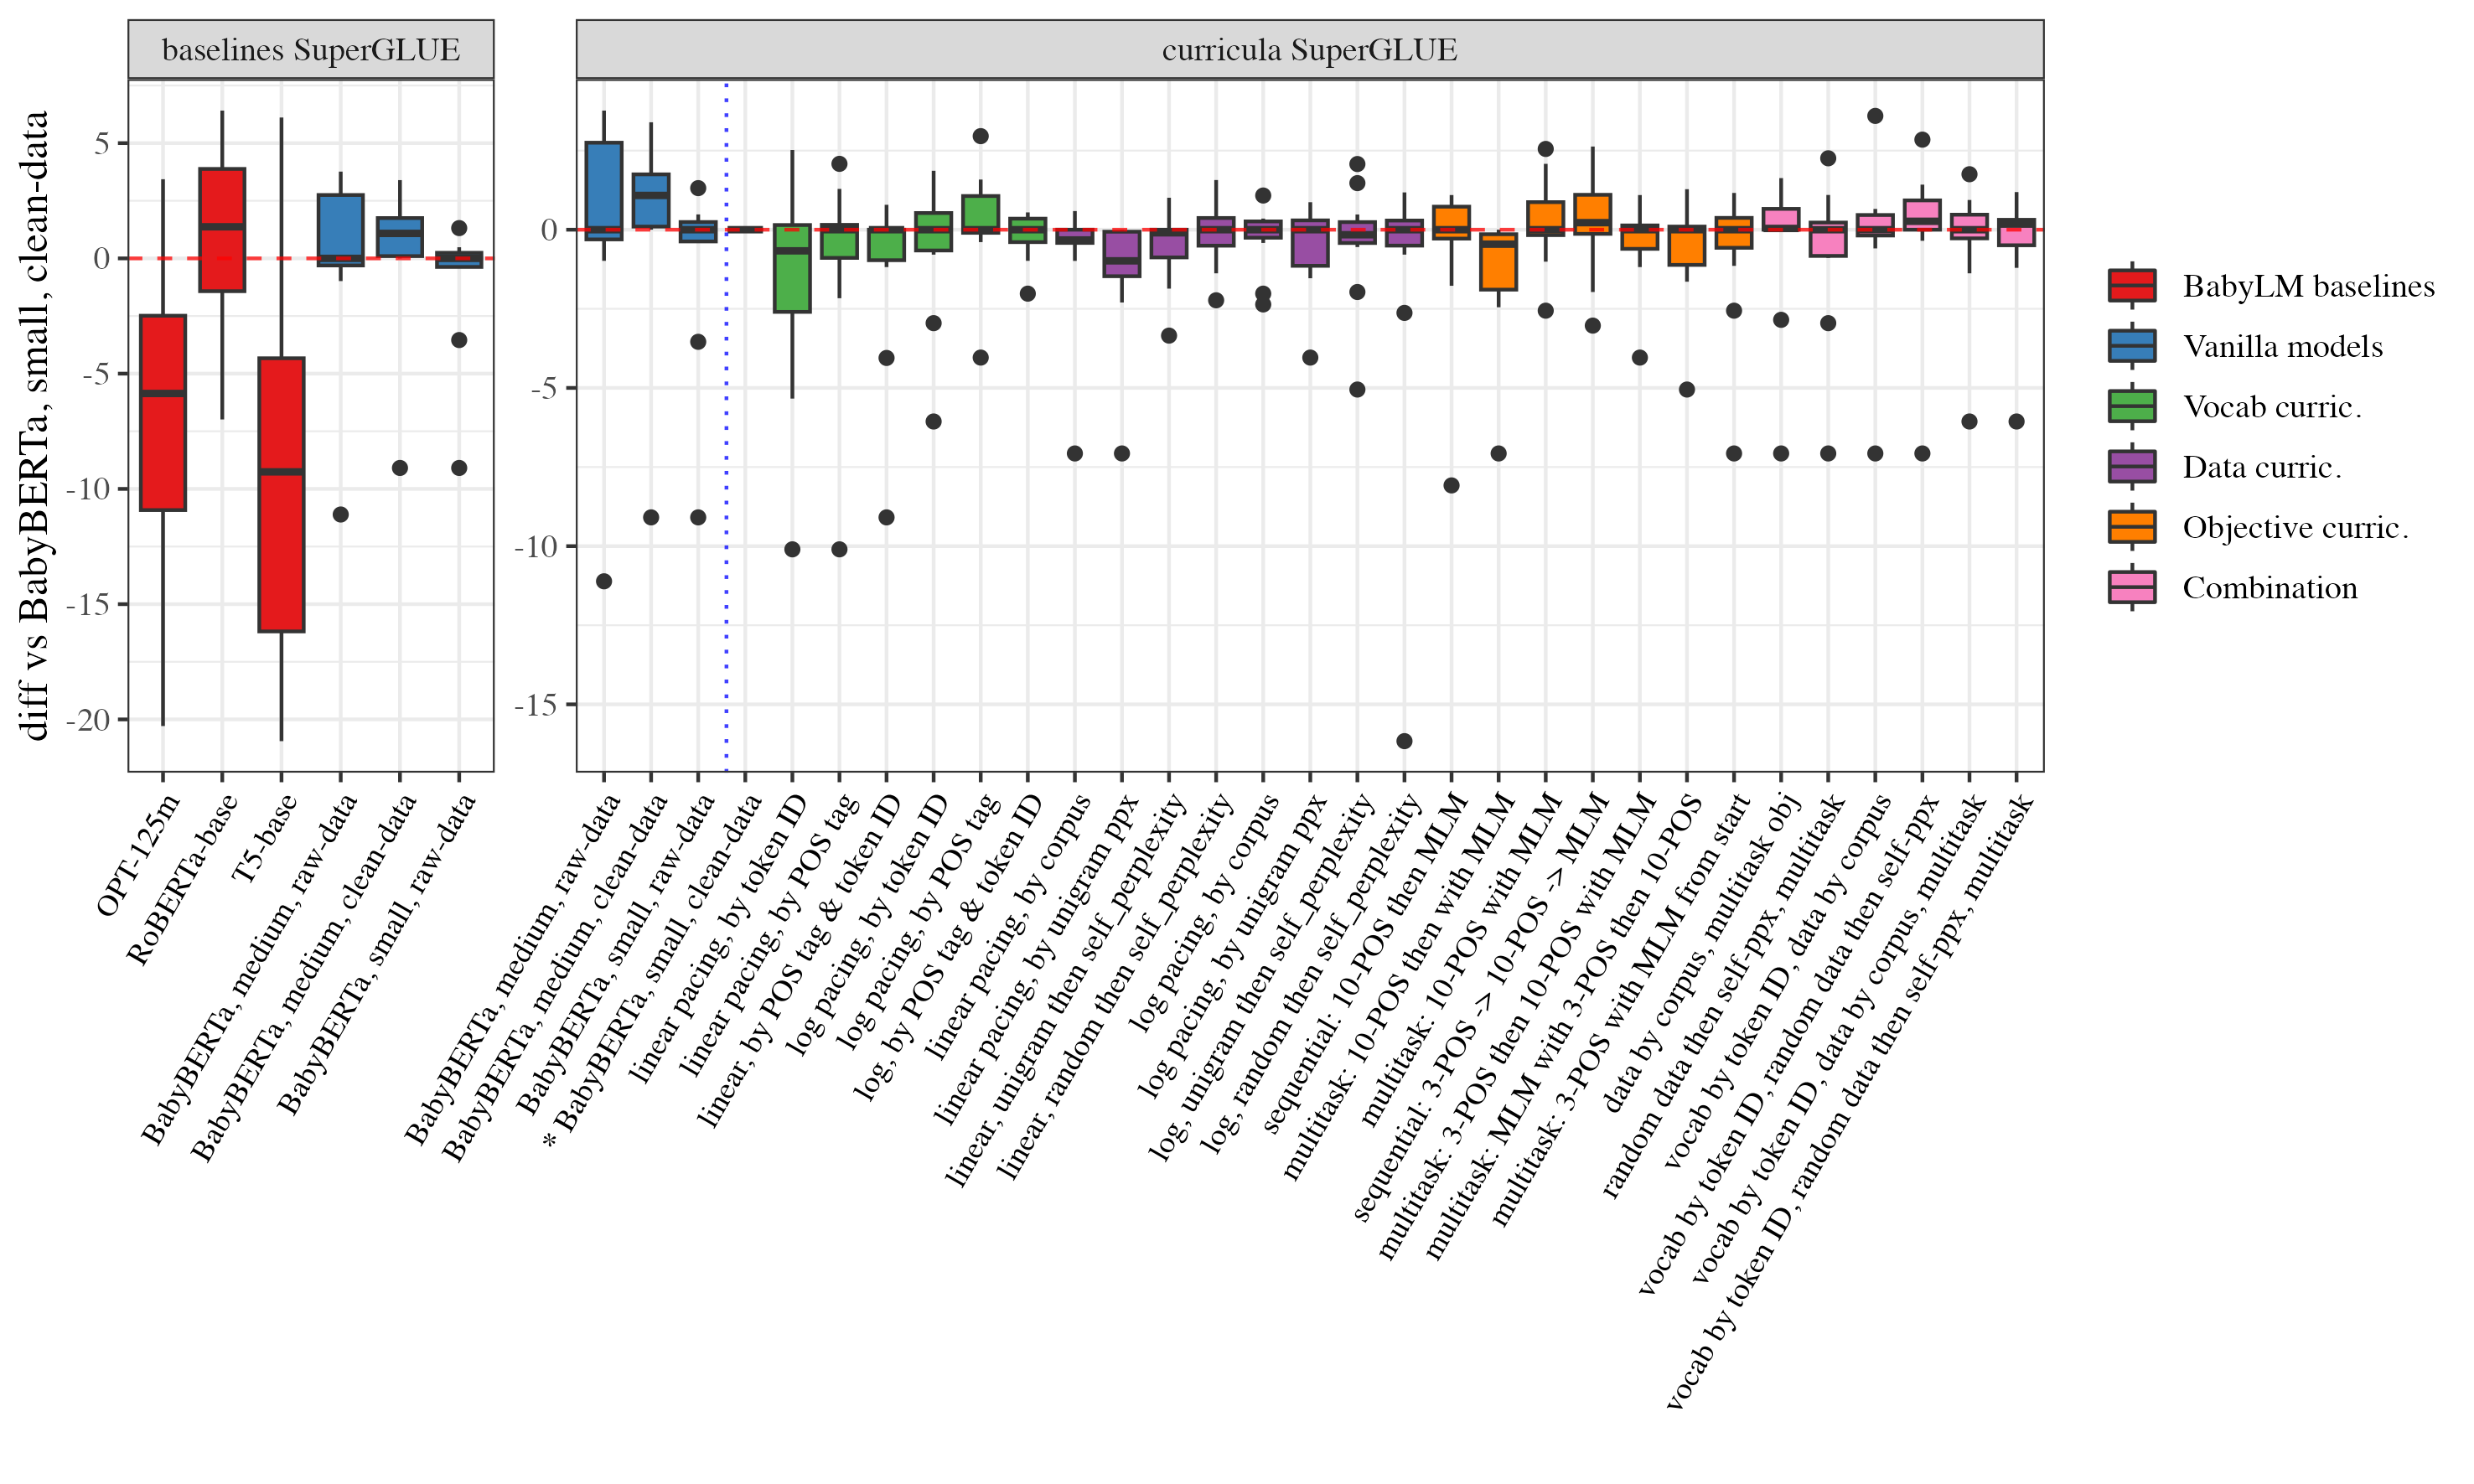
\includegraphics[width=0.9\textwidth]{chapters/climb/figures/babylm_superglue_diffs_boxplots.png}
    \caption{Comparison of model performance across BLiMP (top) and SuperGLUE (bottom) tasks. The plots show the differences in performance between our curriculum learning models and baseline models. Types of curriculum learning are indicated in the legend and highlighted with different colors with explanations in the text.}
    \label{fig:combined-boxplots}
\end{figure}


\section{Results}

Multiple evaluation metrics are employed in BabyLM. In our work, we focus on BLiMP \citep{warstadt2020blimp} and the supplementary BLiMP-style tests provided by the shared task organizers. We also report our results on the natural language understanding benchmark, SuperGLUE \citep{wang2019superglue}, and the ambiguous subset of MSGS (the Mixed Signals Generalization Set) \citep{warstadt2020msgs}. In brief, BLiMP evaluates specific linguistic abilities, MSGS evaluates linguistic preference over surface generalisation and SuperGLUE evaluates downstream task performance. For all scores, we report the average score across all categories, rather than test instances, as provided by the BabyLM evaluation pipeline.\footnote{For instance, there are 12 categories in BLiMP but 50+ individual tests. We average over the scores given for each category, rather than the scores given for each test.} All of our curriculum learning models are small BabyBERTa-style ones using the parameters shown in \cref{tbl:baseline-size-comparison} and the cleaned training dataset of 9.4M words (reduced from the 10M word dataset for the \textsc{strict-small} track) and their results can be found in \cref{tbl:result-vocab-cl}, \cref{tbl:result-data-cl} and \cref{tbl:result-obj-cl}. 


In the tables we compare to our small BabyBERTa-style vanilla model also trained on the clean data (\cref{subsec:baseline}). \cref{fig:combined-boxplots} visualizes these comparisons for the BLiMP and SuperGLUE tasks.

Furthermore, we experimented with some combinations of different curricula to see how they would interact (\cref{tbl:result-combination-cl}). For all of our runs, we use the same set of hyper-parameters that we report in \cref{tbl:baseline_hyperparams}. 


We find notable gains for our own vanilla models over the shared-task baselines, and, while we do not identify further large improvements in our curriculum learning models, we do notice some modest gains which suggest possibilities for future research and experimentation over variables. While the differences in performance between most of our experimental conditions are small, the large number of ablations we run enables us to provide a comprehensive set of recommendations for how and when different curriculum learning strategies may offer improved performance on linguistic tasks. Below we summarize our observations over the full results tables.

\begin{table*}
    \centering
    \small
    % \setlength{\tabcolsep}{3pt}  % Reduce column spacing further
    \begin{tabular}{ll|rrrrr}
    \toprule
    Pacing & Type & PPX & BLiMP & BLiMP.S & GLUE & MSGS \\
    \midrule
    \textsuperscript{\textdagger}Linear & \lightgreenhighlight{Freq} & 9.70 & 75.09 & \textbf{66.43} & 68.71 & 68.61 \\
    Linear & \darkgreenhighlight{POS} & 10.17 & 72.06 & 63.44 & 69.50 & 66.91 \\
    Linear & \verydarkgreenhighlight{Hybrid} & 10.21 & 73.37 & 66.11 & 69.22 & 66.61 \\
    Log & \lightgreenhighlight{Freq} & 9.26 & 74.97 & 64.63 & 69.94 & 66.82 \\
    Log & \darkgreenhighlight{POS} & 9.29 & 74.12 & 62.06 & \textbf{70.66} & \textbf{70.52} \\
    Log & \verydarkgreenhighlight{Hybrid} & 9.29 & 74.74 & 63.62 & 70.29 & 66.42 \\
    \midrule
    Vanilla & & \textbf{9.21} & \textbf{75.48} & 65.34 & 70.47 & 68.30 \\
    \bottomrule
    \end{tabular}
    \caption{\label{tbl:result-vocab-cl} Results for vocabulary curriculum models (\cref{subsec:vocab-cl}). All models score above 90 in the MSGS Control tasks. \textsuperscript{\textdagger} indicates the model we submitted to BabyLM, `CLIMB-tokens'. PPX = Perplexity, BLiMP.S = BLiMP.Supp, GLUE = (Super)GLUE, MSGS = MSGS Ambig.}
\end{table*}
    
We now group our experimental results according to the three curriculum learning approaches: \textbf{vocabulary}, \textbf{data}, and \textbf{objective} curricula. While our curriculum models do not uniformly outperform the vanilla BabyBERTa-style baseline, we do observe small but consistent gains in some areas. These findings point toward useful strategies for future research on curriculum learning in low-resource language modelling.

\subsection{Vocabulary Curriculum}

\paragraph{Different representations of vocabulary difficulty work better for different tasks.}
When representing difficulty in the vocabulary curriculum experiments, token ID -- our proxy for frequency -- appears to work better than word classes (POS tags) or a combination of token ID and POS tags on the BLiMP evaluation tasks, but worse than POS tags on SuperGLUE and MSGS (\cref{tbl:result-vocab-cl}).

\paragraph{Log pacing sometimes helps for vocabulary curriculum learning, but not consistently.}
While log pacing outperforms linear pacing on BLiMP in 2 out of 3 configurations and across all SuperGLUE settings (3/3), it performs worse across the board on the BLiMP Supplement tasks (0/3). This suggests that pacing strategies for vocabulary exposure are task-sensitive. It is possible that the diverse vocabulary required by BLiMP Supplement tasks may not be well captured by our current pacing functions, indicating room for future exploration of more tailored schedules or functions inspired by non-monotonic learning trajectories.

\subsection{Data Curriculum}

\begin{table*}
    \centering
    \small
%    \setlength{\tabcolsep}{3pt}  % Reduce column spacing further
    \begin{tabular}{ll|rrrrr}
    \toprule
    Pacing & Type & PPX & BLiMP & BLiMP.S & GLUE & MSGS \\
    \midrule
    Linear & \lightpurplehighlight{Source} & 10.41 & 73.32 & 61.99 & 69.68 & 66.22 \\
    Linear & \darkpurplehighlight{Static PPX} & 12.51 & 72.45 & 61.67 & 69.10 & 66.90 \\
    Linear & \verydarkpurplehighlight{Dynamic PPX-U} & 11.88 & 72.62 & 62.57 & 69.86 & 66.64 \\
    Linear & \verydarkpurplehighlight{Dynamic PPX-R} & 10.82 & 71.88 & 63.10 & 70.37 & 67.48 \\
    Log \textsuperscript{\textdagger} & \lightpurplehighlight{Source} & \textbf{9.21} & \textbf{75.87} & 64.29 & 70.20 & \textbf{70.99} \\
    Log & \darkpurplehighlight{Static PPX} & 9.39 & 75.03 & 63.78 & 69.90 & 66.69 \\
    Log & \verydarkpurplehighlight{Dynamic PPX-U} & 9.35 & 74.83 & 64.24 & 70.09 & 66.89 \\
    Log & \verydarkpurplehighlight{Dynamic PPX-R} & \textbf{9.21} & 75.81 & 63.03 & 68.93 & 66.64 \\
    \midrule
    Vanilla & & \textbf{9.21} & 75.48 & \textbf{65.34} & \textbf{70.47} & 68.30 \\
    \bottomrule
    \end{tabular}
    \caption{\label{tbl:result-data-cl} Results for data curriculum models (\cref{subsec:data-cl}). All models score above 92 in the MSGS Control tasks. \textsuperscript{\textdagger} indicates the model we submitted to BabyLM, `CLIMB-data-split'. PPX = Perplexity, BLiMP.S = BLiMP.Supp, GLUE = (Super)GLUE, MSGS = MSGS Ambig.}
\end{table*}


\paragraph{In multi-corpora datasets, ordering by difficulty is a good first step.}
Training data requirements have grown so much in modern NLP that usually training a language model from scratch will involve multiple datasets, or multiple domains. The results of our data curriculum experiments indicate that a good first step is to put these sub-corpora into some order of intuitive difficulty, as we did (\cref{tbl:result-data-cl}). In the case of BLiMP this approach outperforms our perplexity-based data curricula, and with log pacing our vanilla model. The same is true of MSGS  (with log pacing), as well as BLiMP-supplement and SuperGLUE (though the last two do not beat our vanilla model). 
Amongst the perplexity-driven models, the picture is less positive: out of 24 tests, only one model outperforms our vanilla model (log pacing, random initialisation + model perplexity in \cref{tbl:result-data-cl}).

\paragraph{Perplexity-driven approaches for data curriculum learning underperform.}
Although perplexity-based ordering intuitively reflects learning difficulty, it proves less effective in our experiments. Across 24 different perplexity-based configurations, only one outperformed our vanilla model (log pacing, random initialization + model perplexity) \cref{fig:baseline_obj_cl_superglue}. This suggests that our perplexity estimates may not capture relevant complexity for the model at small scales, and further work is needed to refine how perplexity is computed or used.


\subsection{Objective Curriculum}
\begin{table*}
    \centering
    \small
    \begin{tabular}{l@{\hspace{-15pt}}lll|rrrrr}
    \toprule
    & \multicolumn{3}{l}{Task duration (\% of training)} & & & & \\
    Type & 3 POS & 10 POS & MLM & PPX & BLiMP & BLiMP.S & S.GLUE & MSGS \\
    \midrule
    \lightorangehighlight{Seq} & -- & 0 - 12.5 & 12.5 - 100 & 9.58  & 73.87 & 62.98      & 69.85       & 66.70    \\
    \darkorangehighlight{MT} & -- & 0 - 100 & 12.5 - 100 & 9.78   & 74.60 & 62.17     & 69.12       & 66.64    \\
    \darkorangehighlight{MT} & -- & 0 - 100 & 0 - 100    & 9.30  & \textbf{75.82} & 65.77     & \textbf{70.74}       & 66.58    \\
    \lightorangehighlight{Seq} & 0 - 6.25 & 6.25 - 12.5 & 12.5 - 100 & 9.49  & 74.03 & 63.02      & 70.71       & 66.93    \\
    \darkorangehighlight{MT} & 0 - 6.25 & 6.25 - 100  & 12.5 - 100 & 9.72  & 73.68 & 63.89     & 70.07       & 67.00    \\
    \darkorangehighlight{MT} \textsuperscript{\textdagger} & 0 - 6.25 & 6.25 - 100  & 0 - 100    &  9.30 & 74.80 & \textbf{67.55}      & 69.89       & 67.65    \\
    \darkorangehighlight{MT} & 0 - 100  & -- & 0 - 100   & 9.25  & 74.48 & 63.98     & 69.77       & 67.72    \\
    \midrule
    Vanilla Model & &  & & \textbf{9.21}  & 75.48 & 65.34 & 70.47 & \textbf{68.30} \\
    \bottomrule
    \end{tabular}
    \caption{\label{tbl:result-obj-cl} Results for objective curriculum models (\cref{subsec:objective-cl}). All models score above 94 in the MSGS Control tasks. Task duration defines when an objective function was active during training, as a percentage of the total number of training steps. \textsuperscript{\textdagger} indicates the model we submitted to BabyLM, `CLIMB-multitask'. }
\end{table*}



\paragraph{Objective curricula, especially multitask setups combining POS tagging with MLM, show clear benefits on syntactic and downstream tasks.} \cref{fig:baseline_obj_cl_blimp_supp} and \cref{fig:baseline_obj_cl_superglue} compare our small BabyBERTa-style vanilla  model to our best objective curriculum learning setting -- a multi-task trained model with sequential POS-tag prediction -- on each task in BLiMP Supplement and (Super)GLUE. We find our curriculum-learning (CL) model outperforms our vanilla model on 5/6 tasks in BLiMP Supplement. While on (Super)GLUE, our CL model outperforms our baseline on 4/10 tasks and obtains comparable performance on another 4/10 tasks. This results illustrate the potential to further explore objective-curricula settings.


\begin{figure}[h]
    \centering
    \begin{subfigure}[b]{0.48\textwidth}
        \centering
        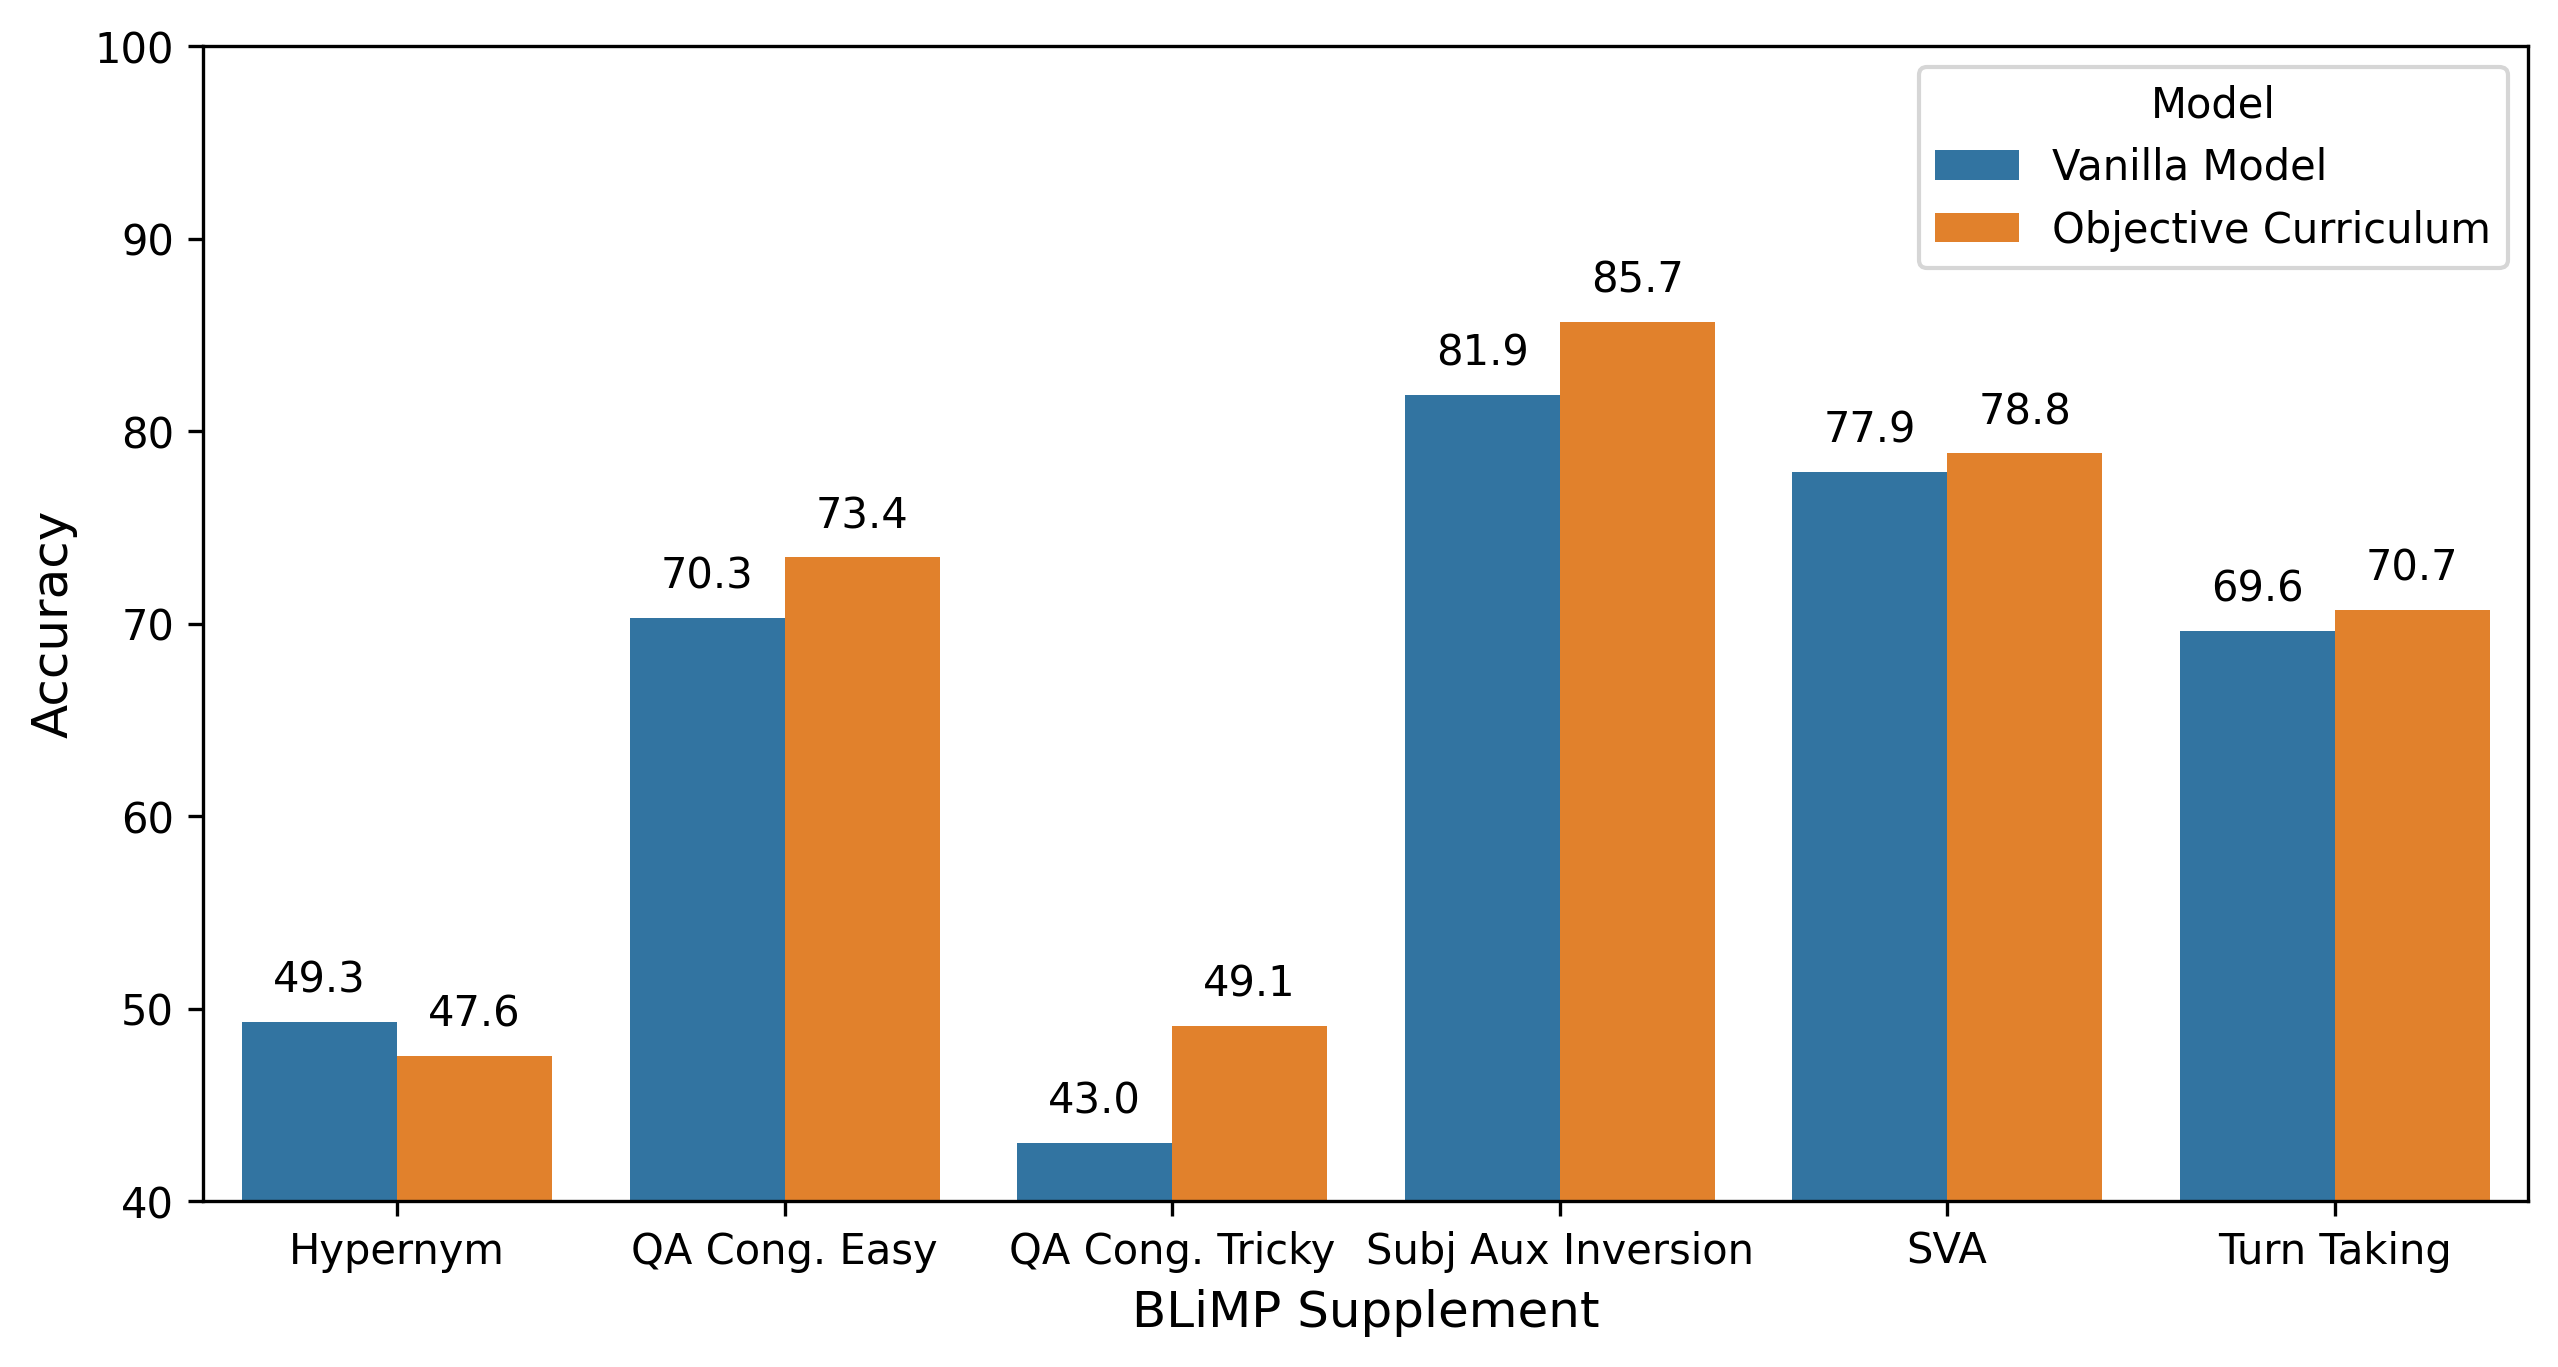
\includegraphics[width=\textwidth]{chapters/climb/figures/baseline_vs_obj_cl_blimp_supp_new.png}
        \caption{BLiMP supplementary tasks}
        \label{fig:baseline_obj_cl_blimp_supp}
    \end{subfigure}
    \hfill
    \begin{subfigure}[b]{0.48\textwidth}
        \centering
        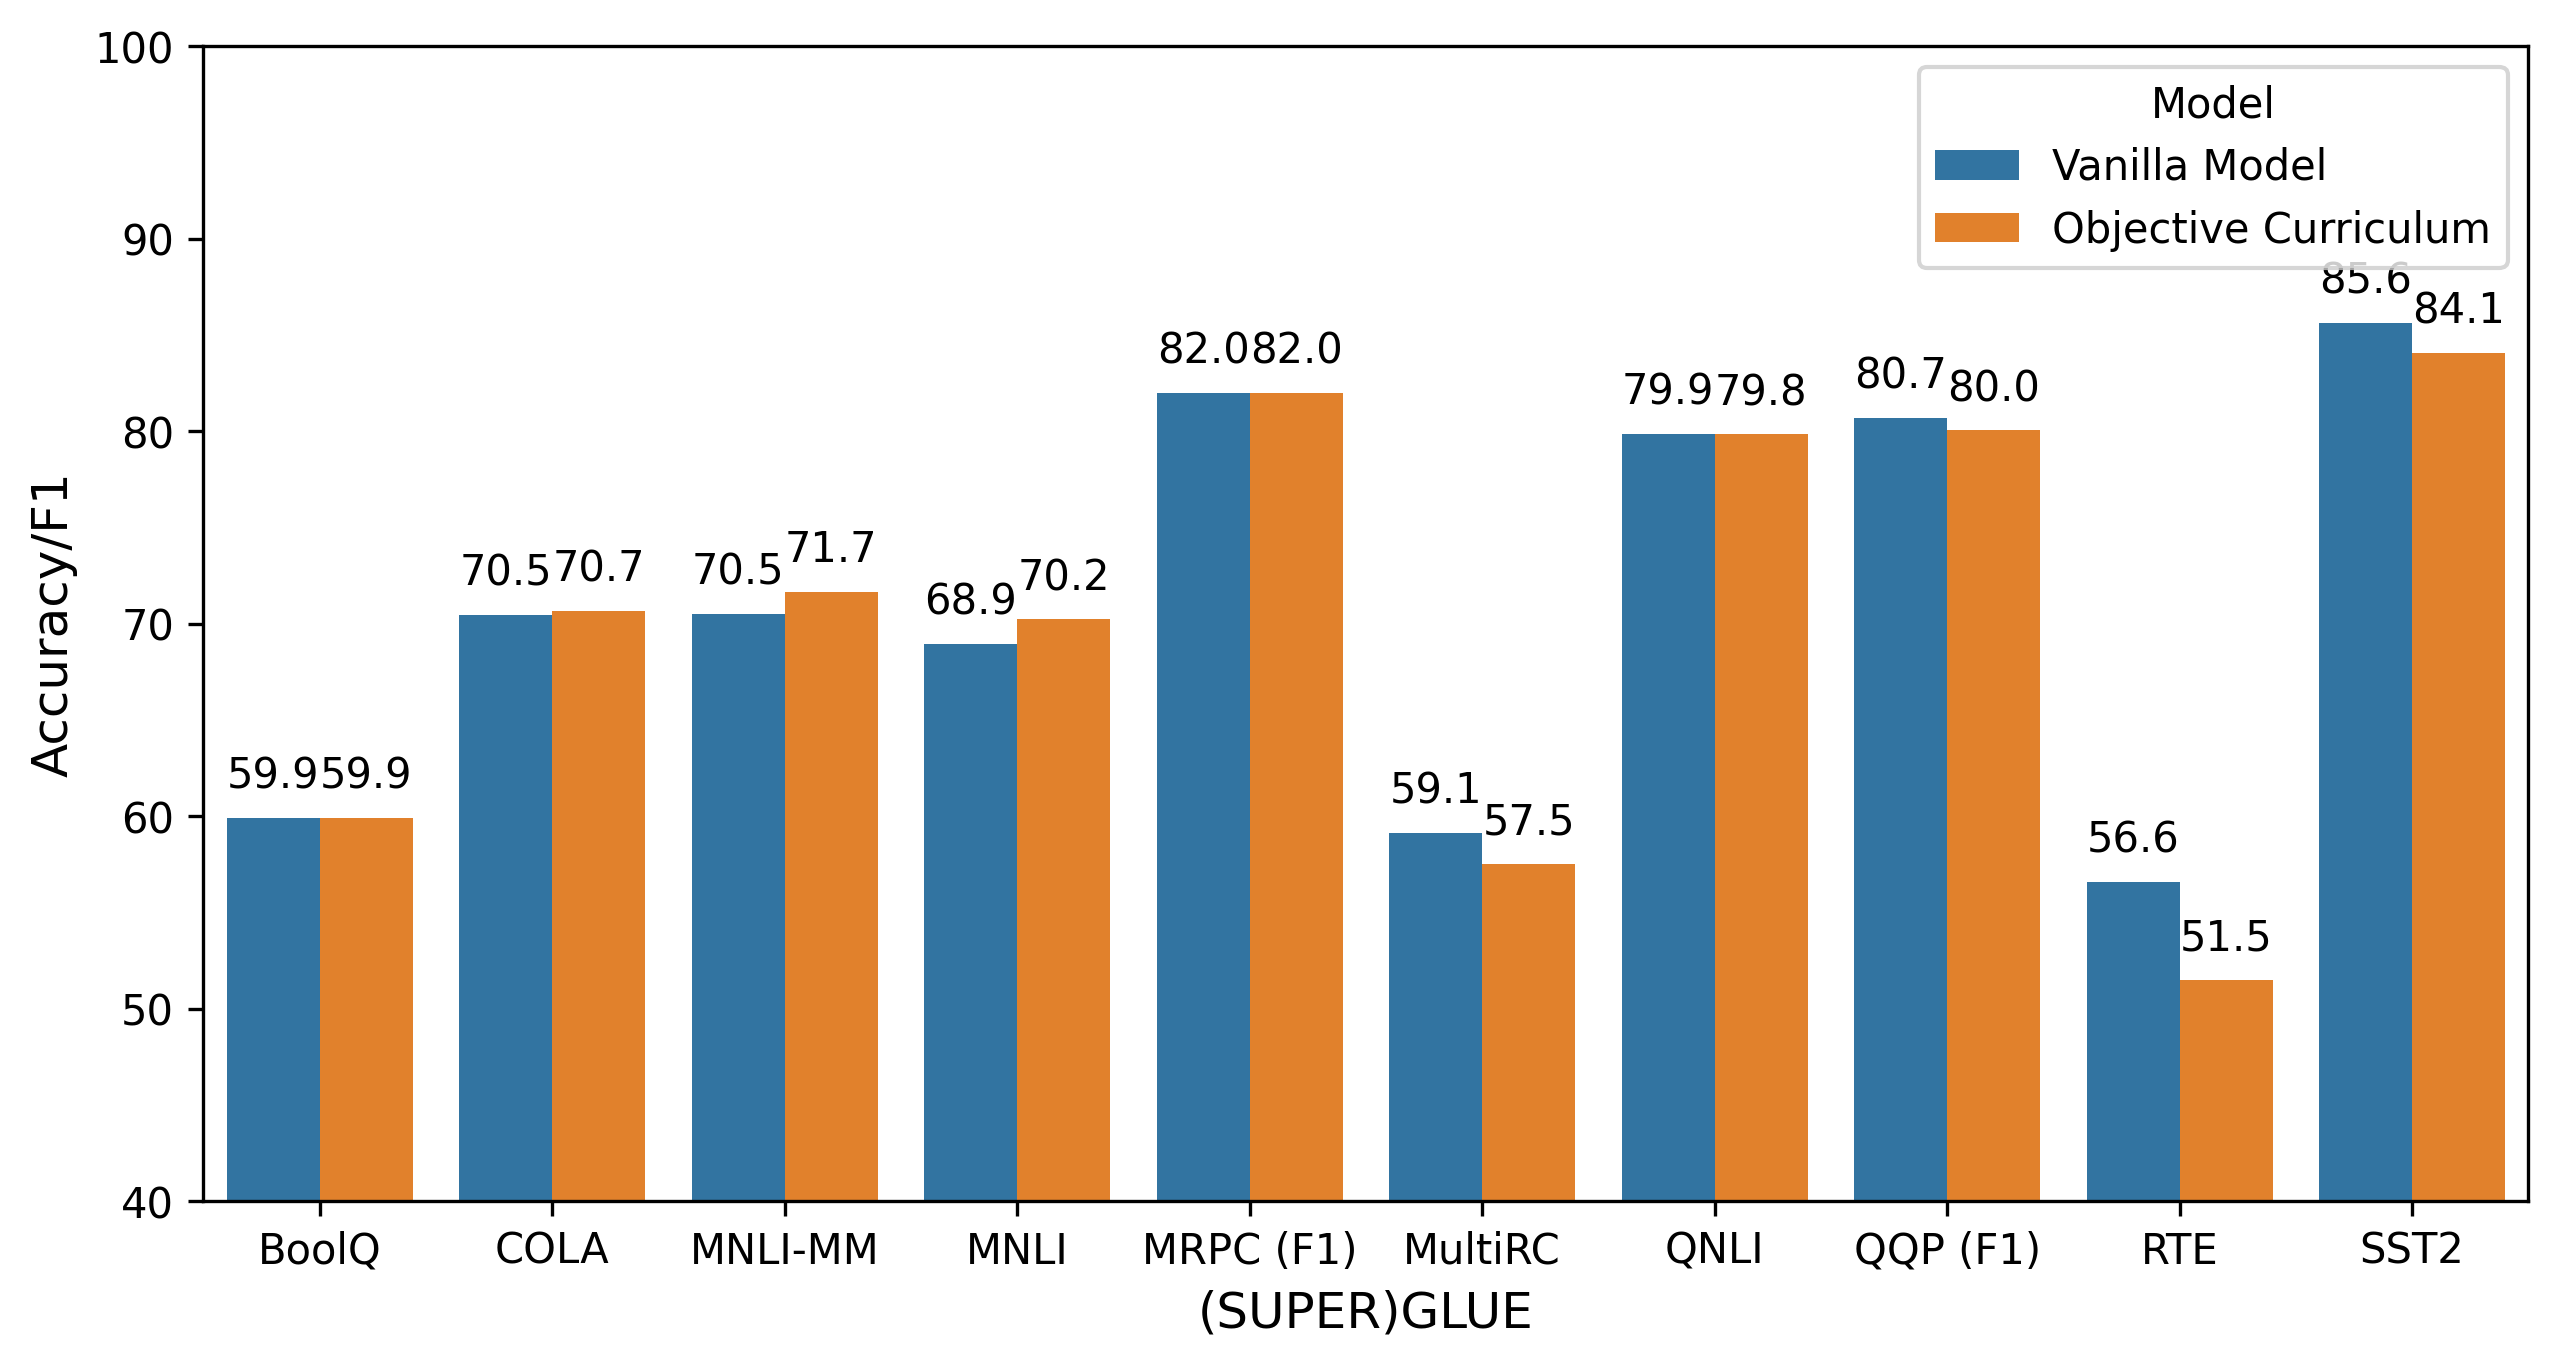
\includegraphics[width=\textwidth]{chapters/climb/figures/baseline_vs_obj_cl_superglue.png}
        \caption{(Super)GLUE tasks}
        \label{fig:baseline_obj_cl_superglue}
    \end{subfigure}
    \caption{Comparison between our vanilla model and the best objective curriculum learning setting on different benchmark tasks.}
    \label{fig:baseline_obj_cl_comparison}
    \end{figure}

We also experimented with curriculum learning via variation in training objectives. These include sequential curricula (where objectives are swapped at fixed training stages) and multitask learning setups (where multiple objectives are trained jointly).

\paragraph{Multitask learning holds sway over sequentially swapping objective functions for now.}
In our experiments with curricula for the objective function, we compare training on simultaneous tasks -- known as multitask learning \cite{caruana1997multitask} -- with predefined sequences of objective functions which swap from one to another at set thresholds in the training process. We set up two sequential curricula: one with 2 tasks (predicting the 10 universal POS tags found in our dataset, and MLM) and the other with 3 (like the 2 task curriculum, additionally with noun/verb/other prediction). We compare these against multitasking alternatives. In general the sequential curricula are outperformed by the multitasking ones, though the 3-task sequential curriculum outperforms our BabyBERTa-style vanilla model on SuperGLUE and is second only marginally to our best-performing multitask model (\cref{tbl:result-obj-cl}). The multitask learning model with 10-class universal POS-tag prediction and MLM in place from the outset performs best on BLiMP and SuperGLUE. However, our best model on BLiMP-supplement -- a multitask one -- has an element of sequential task scheduling in that the two POS-tag prediction tasks are lined up one after the other, with a switch from 3-class to 10-class after 6.25\% of training steps. In \cref{fig:baseline_obj_cl_blimp_supp}, we visualize this result for each task in BLiMP-supplement, illustrating that our curriculum learning model improves over our vanilla model in 5/6 tasks.
Altogether, these results suggest that sequential objective function curricula do hold some potential for performance gains if further tuning of the tasks and scheduling can be carried out.

\paragraph{Sequential training has potential with tuning.}
Although multitask learning tends to dominate, some sequential objective curricula also perform well. In particular, a 3-task curriculum (noun/verb/other POS prediction $\rightarrow$ 10-class POS $\rightarrow$ MLM) yields strong performance on SuperGLUE and is only narrowly behind the multitask version. These results indicate that sequential curricula may offer further benefits if task timing and transitions are more carefully optimised.

\paragraph{Objective structure aids syntactic generalization.}
Models incorporating POS objectives---either in multitask or sequential form---often outperform vanilla models on BLiMP Supplement, which tests syntactic sensitivity. This supports the idea that structured auxiliary objectives guide the model toward syntactic generalisation, and could be explored further for syntactic evaluation tasks.


\subsection{Combined Curricula and Additional Observations}

\paragraph{In general, log pacing works at least as well as linear pacing across different curricula learning strategies.}
In our data curriculum experiments, models using the log pacing function outperform their linear counterparts in 4/4 settings on BLiMP, and 3/4 settings for BLiMP-supplement and SuperGLUE (\cref{tbl:result-data-cl}). This indicates that rapidly increasing the difficulty of training instances in the early stages brings downstream benefits on grammaticality and NLU tasks.

In our vocabulary curriculum experiments on the other hand, there is not such a clear picture. Log pacing outperforms linear in 2/3 settings on BLiMP and 3/3 on SuperGLUE, but 0/3 for BLiMP-supplement (\cref{tbl:result-vocab-cl}).
Presumably this is a reflection of the different vocabulary required by each set of evaluation tasks, which could be a matter for future investigation but also indicates that we do not yet have a clear generalizable pacing function for the vocabulary curriculum. There are of course other pacing functions to be tried.

\begin{table*}
    \centering
    \small
    \begin{tabular}{l@{\hspace{-10pt}}ll|rrrrr}
    \toprule
    Vocab \ & Data \ & Objective \ & PPX & BLiMP & BLiMP.S & S.GLUE & MSGS  \\
    \midrule
    -- & \lightpurplehighlight{Source} & \darkorangehighlight{MT} &                           9.29& 74.06 & 64.06 & 70.02 & 66.90 \\
    -- & \verydarkpurplehighlight{Dynamic PPX-R} & \darkorangehighlight{MT} &                9.44& 75.89 & 64.63 & 69.72 & 67.78 \\
    \lightgreenhighlight{Freq} & \lightpurplehighlight{Source} & -- &                     9.27& 75.89 & 64.62 & 70.24 & 67.90 \\
    \lightgreenhighlight{Freq} & \verydarkpurplehighlight{Dynamic PPX-R} & -- &        9.30& 75.88 & \textbf{65.79} & 70.42 & 66.63 \\
    \lightgreenhighlight{Freq} & \lightpurplehighlight{Source} & \darkorangehighlight{MT} &         9.22 & 74.86 & 62.82 & 70.09 & 66.68 \\
    \lightgreenhighlight{Freq} & \verydarkpurplehighlight{Dynamic PPX-R} & \darkorangehighlight{MT} & 9.46& \textbf{75.92} & 63.68 & 69.98 & \textbf{71.30} \\
    \midrule
    Vanilla Model & & & \textbf{9.21} & 75.48 & 65.34 & \textbf{70.47} & 68.30 \\
    \bottomrule
    \end{tabular}
    \caption{\label{tbl:result-combination-cl} Results for the combination curriculum models. The multitask objective curriculum refers to the 2-task 10-POS and MLM model shown in \cref{tbl:result-obj-cl}. }
\end{table*}

\paragraph{Combining all three curricula shows potential on BLiMP.}
While each individual curriculum learning experiment did not result in consistent improvements across tasks, we investigated whether combining aspects from the different curricula would, together, improve the model.
We do find that a combination of all three curricula outperforms any single curriculum model on BLiMP, but the same is not true for BLiMP-supplement and SuperGLUE (\cref{tbl:result-combination-cl}). This is another matter for future investigation, as it seems that improving each of the three curricula we investigate may lead to further gains if they are all combined.


\paragraph{In small data settings, filtering data which we intuitively think is noisy is in fact counter-productive.} Perhaps surprisingly, we find that the vanilla models trained on the raw data outperform those trained on the pre-processed data on BLiMP and MSGS. We surmise that models can learn even from linguistically non-standard datapoints.

\section{Discussion}\label{sec:discussion}

We set out to investigate a number of curriculum learning approaches to language model training, motivated by findings from the human language acquisition process and by the wish to successfully train smaller models for smaller budgets.
We first of all implemented a stronger model of our own, based on BabyBERTa \cite{huebner2021babyberta} and found that a small 8-layer vanilla model could outperform the provided BabyLM baselines on the BLiMP grammaticality tests and get close to the best RoBERTa shared-task baseline on SuperGLUE. This underlines the findings reported in the BabyBERTa paper: that with smaller datasets, it makes sense to use smaller models and a smaller vocabulary size.

The results of our curriculum learning experiments, trained with a small BabyBERTa-style vanilla model, suggest that we can further improve performance in certain linguistic tasks by careful application of a pacing function, how we represent and grow the model's vocabulary during training, select the next training instances according to their difficulty, and vary the objective function. Specifically, we find that a logarithmic pacing function works better for the data curriculum than a linear one, but the findings for the vocabulary curriculum are less clear. Other pacing functions might be tried in the future, including those that reflect acquisition theory around non-monotonic or `U-shaped' development trajectories.

It is apparent that ordering the subcorpora within a training set may be worthwhile, and that perplexity-based approaches to data selection hold potential even though we have not found a clear-cut best method for perplexity calculation as yet. As shown in other NLP work, multitask learning can be a beneficial approach, though MLM or next-word prediction remain preeminent as singular tasks used in language modeling. We find multitask learning models hard to beat in the objective curriculum, but do find good performance in our sequential settings. We believe that future work varying the timing of task switches and introducing more tasks could be worthwhile.

On a more general note, the Baby LM challenge evaluates a language model only on its final downstream performance on a set of tasks -- i.e.\ at a finite point in time. The challenge does not directly measure whether a given model is learning in a `human-like' fashion. Our contribution to the BabyLM challenge is to provide a set of curriculum learning strategies which are motivated by the language learning dynamics of infants and children. We encourage future research to study how to quantitatively evaluate whether the learning trajectory of a model parallels that of a human language learner and how similarities to human language learning results in downstream NLU performance. 


\section{Conclusions}

This chapter explored how principles from child language acquisition can guide the structure and pacing of language model training. Specifically, we implemented three curriculum learning strategies inspired by human development: gradually increasing vocabulary size (\textbf{vocabulary curriculum}), ordering training data by intuitive or model-based difficulty (\textbf{data curriculum}), and varying the specificity of the objective function over time (\textbf{objective curriculum}).

Across these experiments, we found that our BabyBERTa-style vanilla models already outperform the BabyLM baselines on BLiMP and MSGS, and perform competitively on SuperGLUE. Curriculum learning approaches offer modest but consistent gains in some areas, particularly when using log pacing functions, source-based data ordering, or multitask objectives. These results suggest that developmental structure in training can yield benefits even in resource-constrained settings.

Notably, models trained on raw, unfiltered data often outperformed those trained on cleaned data, reinforcing the idea that early exposure to linguistic variation (even with noisy data)may help small models generalize better, much like children learning from diverse, real-world input.

Beyond specific gains, this chapter establishes a computational framework for implementing curriculum learning strategies aligned with cognitive development. In doing so, it addresses the macro-level question posed at the start of this thesis: \textit{can language models benefit from learning more like humans do, by following a structured, developmentally inspired trajectory?} 

The next chapter builds on this foundation by shifting focus to the micro-level dynamics of representation. There, we introduce \smoothing, a method motivated by how children use grammatical context to infer word meaning. While \climb explored how to structure the learning experience, \smoothing investigates how to shape internal representations to support better generalization from limited exposure.


% \begin{table*}
% \centering
% \small
% \begin{tabular}{llrrrrr}
% \toprule
% Type              & Model    & PPX   & BLiMP & BLiMP.Supp & (Super)GLUE & MSGS Ambig \\
% \midrule
% Official Baseline & OPT-125m         & --    &   63.16 & 55.08 & 63.38 & 69.22 \\
%                   & RoBERTa-base      & --  &   
%                 69.84 & 50.52 & 71.42 & 70.25 \\
%                   & T5-base         & --    &   58.27 & 47.55  & 60.93 & 68.55 \\
% \midrule
% Vanilla Models    &CLIMB-base (medium)   & 9.01   & 75.66 & 66.13 & 70.75 & 67.62 \\
%                   & CLIMB-base-small & 9.21  & 75.48 & 65.34 & 70.47 & 68.30 \\
%                   & CLIMB-raw (medium)   &  8.47   & 77.97 & 66.16 & 70.63 & 69.44 \\
%                   & CLIMB-small-raw  & 8.64  & 76.42 & 64.60 & 69.46 & 70.65 \\
%                 & \emph{large-100M}      & 4.35      &   81.03 & 75.56 & 72.93 & 74.17 \\
% \midrule
% Vocab Curriculum          & CLIMB-tokens   &  9.70  & 75.09 & 66.43  & 68.71 & 68.61 \\
% Data Curriculum           & CLIMB-data-split & 9.21 & 75.87 & 64.29  & 70.20 & 70.99 \\
% Objective Curriculum      & CLIMB-multitask & 9.30 & 74.80 & 67.55  & 69.89 & 67.65 \\
% \bottomrule
% \end{tabular}
% \caption{\label{tbl:submission-comparison} Comparison between the official shared task baselines, our BabyBERTa-style vanilla models, and our submitted curriculum learning models on the main evaluation tasks: BLiMP, (Super)GLUE, and MSGS. Our *small and *medium models are defined in Section \ref{subsec:baseline}. All models are trained on pre-processed data except for those labelled with *-raw, which are trained on mostly unprocessed data (except we join the input sentences). The `large-100M' model was a larger BabyBERTa-style model trained on the 100M BabyLM training set (all others have been trained on the 10M dataset available in the \textsc{strict-small} track). }
% \end{table*}


% --- Additional Stuff ---

% \subsection{Curriculum Learning Approach}
% Our work introduces curriculum learning to three primary components of language model pre-training: vocabulary (Section \ref{subsec:vocab-cl}), data sampling approach (Section \ref{subsec:data-cl}), and objective function selection (Section \ref{subsec:objective-cl}). This multi-faceted approach is inspired by how humans learn language, where different aspects of language acquisition develop simultaneously but at different rates. For each component, we implement dynamic difficulty scaling that evolves over the course of training, simulating the progressive nature of human language learning. The specific variables and configurations for each curriculum learning experiment are detailed in Table~\ref{tbl:configurations}.

% \begin{table*}
%     \centering
%     \small
%     \begin{tabular}{llc}
%     \toprule
%          Type & Model & Training Time \\
%     \midrule
%          Vanilla Models & CLIMB-small-raw & 12h \\
%          & CLIMB-raw (medium) & 17h40m \\
%     \midrule
%          Data Curriculum & Log Source & 12h30m \\
%          & Log Random + model ppl & 17h10m \\
%          Objective Curriculum & Sequential All POS & 11h40m \\
%          & Multitask All POS & 15h30m \\
%          Vocabulary Curriculum & Linear POS & 11h50m \\
%          & Log Token ID & 12h10m \\
%     \midrule
%         Combination & Log Data Split + Log Token ID & 12h30m \\
%         & Log Random + model ppl + Log Token ID & 17h10m \\
%     \bottomrule
%     \end{tabular}
%     \caption{Compute required to train our models. We report the model with the shortest and longest runtime for each experiment type. Each model is trained for 400,000 steps with 4 A100 GPUs.}
%     \label{tbl:compute}
% \end{table*}